\documentclass{article}
\usepackage{amsmath}
\usepackage{graphicx}
\usepackage{lscape}

\usepackage{listings}
\usepackage{xcolor}

% Define custom colors
\definecolor{dkgreen}{rgb}{0,0.6,0}
\definecolor{gray}{rgb}{0.5,0.5,0.5}
\definecolor{mauve}{rgb}{0.58,0,0.82}

% Configure lstlisting settings for Python
\lstset{
  frame=tb,                      % Draw a frame at the top and bottom of the code block
  language=Python,               % Set the language to Python
  aboveskip=3mm,                 % Add space above the code block
  belowskip=3mm,                 % Add space below the code block
  showstringspaces=false,        % Do not display string spaces with special underlines
  columns=flexible,              % Allow flexible column spacing
  basicstyle={\small\ttfamily},  % Set the font style and size for code
  numbers=left,                  % Display line numbers on the left
  numberstyle=\tiny\color{gray}, % Style for line numbers
  keywordstyle=\color{blue},     % Style for keywords
  commentstyle=\color{dkgreen},  % Style for comments
  stringstyle=\color{mauve},     % Style for strings
  breaklines=true,               % Allow long lines to break
  breakatwhitespace=true,        % Break lines at whitespace if possible
  tabsize=4                      % Set tab size to 4 spaces
}


\begin{document}

\section*{\hspace{4cm}\textbf{Lab 1 Assignment}}

\section{Solution to 1(i)}

We can see from the contour that the following function: 
\[
f(x, y) = x^2\left(4 - 2.1x^2 + \frac{1}{3}x^4\right) + xy + y^2\left(-4 + 4y^2\right).
\] 
exhibits some symmetry. To confirm, we check if it's symmetric about the origin. We replace \(x \to -x\) and \(y \to -y\):
\[
f(-x, -y) = (-x)^2\left(4 - 2.1(-x)^2 + \frac{1}{3}(-x)^4\right) + (-x)(-y) + (-y)^2\left(-4 + 4(-y)^2\right).
\]

Simplifying, we have:
\[
f(-x, -y) = x^2\left(4 - 2.1x^2 + \frac{1}{3}x^4\right) + xy + y^2\left(-4 + 4y^2\right),
\]
\[
f(-x, -y) = f(x, y).
\]

The mentioned stationary points in the material are:
\[
x_1 = [0, 0], \quad x_2 = [0.08984201, -0.7126564], \quad x_3 = [1.23022988, 0.16233458].
\]
Since the function \(f(x, y)\) is symmetric about the origin (\(f(-x, -y) = f(x, y)\)), the remaining stationary points are:
\[
x_4 = [-0.08984201, 0.7126564], \quad x_5 = [-1.23022988, -0.16233458].
\]

Thus, the complete set of stationary points is:
\[
x_1 = [0, 0], \quad x_2 = [0.08984201, -0.7126564], \quad x_3 = [1.23022988, 0.16233458],
\]
\[
x_4 = [-0.08984201, 0.7126564], \quad x_5 = [-1.23022988, -0.16233458].
\]


\begin{landscape}
\begin{table}[h!]
\centering
\begin{tabular}{|c|c|c|c|}
\hline
\textbf{Stationary Point \(x_i\)} & \textbf{Hessian Matrix} & \textbf{Eigenvalues of \(H\)} & \textbf{Classification} \\
\hline
\( x_1 = [0, 0] \) & \( \begin{bmatrix} 8 & 1 \\ 1 & -8 \end{bmatrix} \) & \( [8.06225775, -8.06225775] \) & Saddle Point \\
\hline
\( -x_1 = [0, 0] \) & \( \begin{bmatrix} 8 & 1 \\ 1 & -8 \end{bmatrix} \) & \( [8.06225775, -8.06225775] \) & Saddle Point \\
\hline
\( x_2 = [0.08984201, -0.7126564] \) & \( \begin{bmatrix} 7.79724752 & 1 \\ 1 & 16.37819893 \end{bmatrix} \) & \( [7.68225142, 16.49319503] \) & Local Minimum \\
\hline
\( -x_2 = [-0.08984201, 0.7126564] \) & \( \begin{bmatrix} 7.79724752 & 1 \\ 1 & 16.37819893 \end{bmatrix} \) & \( [7.68225142, 16.49319503] \) & Local Minimum \\
\hline
\( x_3 = [1.23022988, 0.16233458] \) & \( \begin{bmatrix} -7.23355211 & 1 \\ 1 & -6.73507924 \end{bmatrix} \) & \( [-8.01490716, -5.95372419] \) & Local Maximum \\
\hline
\( -x_3 = [-1.23022988, -0.16233458] \) & \( \begin{bmatrix} -7.23355211 & 1 \\ 1 & -6.73507924 \end{bmatrix} \) & \( [-8.01490716, -5.95372419] \) & Local Maximum \\
\hline
\end{tabular}
\caption{Classification of Stationary Points}
\end{table}
\end{landscape}


\begin{table}[htbp]
\centering
\begin{tabular}{|c|c|c|c|l|}
\hline
\textbf{Point} &  \textbf{Nature} & \textbf{Reason} \\
\hline
1  & Local Minima  & Surrounded by increasing closed contour lines \\
\hline
2  & Local Minima  & Symmetric nature of the function \\
\hline
3  & Local Maxima & Originally Provided and found through eigenvalues\\
\hline
4 & Local Maxima  & Symmetric nature of the function \\
\hline
5  & Saddle Point  & Originally Provided and found through eigenvalues \\
\hline
6  & Local Minima  & Surrounded by increasing closed contour lines \\
\hline
7  & Local Minima &  Originally Provided and found through eigenvalues \\
\hline
8  & Saddle Point  & Symmetric to Point 9 \\
\hline
9  & Saddle Point  & Forms ridge/valley between two basins of minima \\
\hline
\end{tabular}
\caption{Classification of Stationary Points}
\label{tab:stationary-points}
\end{table}



\begin{figure}[h]
    \centering
    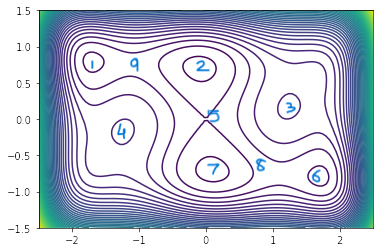
\includegraphics[width=1\textwidth]{lab1c}
    \caption{Stationary Points In Contour Plot}
    \label{lab1c}
\end{figure}

\begin{figure}[h]
    \centering
    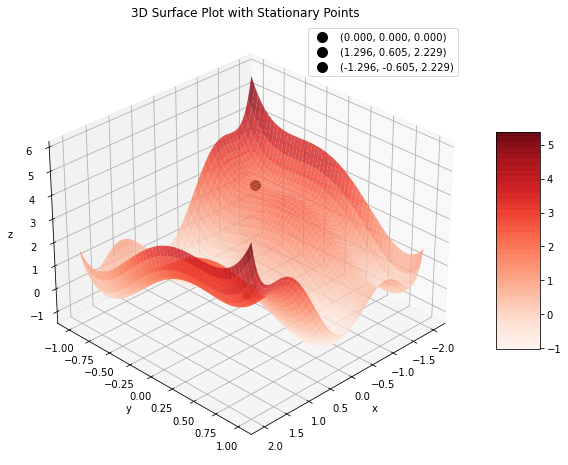
\includegraphics[width=1\textwidth]{lab1p.png}
    \caption{Surface Plot}
    \label{lab1p}
\end{figure}
\begin{enumerate}
    

 \item The image shows the stationary points marked as \( 1,2,3,4,5,6,7,8, 9\) out of which \(3,5,7\) were provided in the lab sheet and \(2,4\) were found due to the symmetric nature of the function. 

 \item Points surrounded by closed contour lines indicate that they are local minima or maxima. If the contours increase in value as we move away from the point, then it is a local minimum and if it decreases then it is a local maxima. Therefore \(1,6\) are stationary points too which are minima. 

 \item  Point \(9\) appears to be a ridge or a valley between two basins of minima. We can say that it is a stationary point (a saddle point). And by symmetry \(8\) is also a saddle point. Sorry the hand script of \(8\) in blue is slightly towards left. It in principle is exactly symmetric to point \(9\). 
 
 \item We can take visual aid of figure  \ref{lab1p} with figure \ref{lab1c} to infer about how the arguments for stationary points develop. By varying the azimuthal angle or rotating the figure we can get further insights through observation supporting points 1,2,3.
 
\end{enumerate}
\newpage
\section{Solution to 1(j)}

\begin{lstlisting}
#importing libraries, functions, hints, decorators (donot affect the runtime).
import numpy as np
import matplotlib.pyplot as plt
from typing import Tuple, List
from dataclasses import dataclass
from ex13func import ex13 as func


@dataclass
class TA_Parameters:
    """We define a class to store parameters for the Taylor approximation."""
    x0: float
    y0: float
    mesh_min: Tuple[float, float] = (-1.5, -1.5)
    mesh_max: Tuple[float, float] = (1.5, 1.5)
    points: int = 1000


def create_mesh(params: TA_Parameters) -> Tuple[np.ndarray, np.ndarray, np.ndarray]:
    """Mesh Generation for plot from the instances of the class."""
    x = np.linspace(params.mesh_min[0], params.mesh_max[0], params.points)
    y = np.linspace(params.mesh_min[1], params.mesh_max[1], params.points)
    return np.meshgrid(x, y)

def compute_taylor_approximation(X: np.ndarray, Y: np.ndarray,
                                 params: TA_Parameters,
                                 func) -> Tuple[np.ndarray, np.ndarray]:
    """
    Compute original function and its Taylor approximation.

    Args:
        X, Y: Mesh Grids
        params: TA_Parameters instance
       ex13: Function to approximate

    Returns:
        Tuple of (exact function value, Taylor approximated value)
    """

    # Original function
    Z =func(0, X, Y)

    # Taylor approximations
    f =func(0, [params.x0, params.y0])
    g = func(1, [params.x0, params.y0])
    H = func(2, [params.x0, params.y0])


    X1 = X - params.x0
    Y1 = Y - params.y0

    # Taylor Polynomial
    ZT = (f +
          g[0] * X1 +
          g[1] * Y1 +
          0.5 * H[0][0] * X1 * X1 +
          H[0][1] * X1 * Y1 +
          0.5 * H[1][1] * Y1 * Y1)

    return Z, ZT

def plot_contours(X: np.ndarray, Y: np.ndarray,
                  Z: np.ndarray, ZT: np.ndarray,
                  params: TA_Parameters) -> None:
    """
    Generate Contours
    Args:
        X, Y: Mesh Grids
        Z: Exact function value
        ZT: Taylor approximation value
        params: TA_Parameters instance
    """

    fig, ax = plt.subplots(figsize=(10, 8))
     # Plot original function contours
    cp1 = ax.contour(X, Y, Z, 50, cmap=plt.get_cmap('hsv'))
    # Plot Taylor approximation contours
    cp2 = ax.contour(X, Y, ZT, 50, cmap=plt.get_cmap('plasma'))

    # Add labels and title
    ax.set_xlabel('x')
    ax.set_ylabel('y')
    ax.set_title(f'Contour Plot with Taylor Approximation\n(x₀={params.x0}, y₀={params.y0})')

    # Add color bar for Taylor approximation
    plt.colorbar(cp2, ax=ax, label='Taylor Approximation')
    # Mark the approximation point
    ax.plot(params.x0, params.y0, 'r*', markersize=10,
            label='Approximation Point')

    ax.legend()
    plt.show()

def main():
    """Main function to run the visualization."""
    params = TA_Parameters(x0=0, y0=0.5)
    X, Y = create_mesh(params)
    Z, ZT = compute_taylor_approximation(X, Y, params, ex13)
    plot_contours(X, Y, Z, ZT, params)

if __name__ == "__main__":
    main()



\end{lstlisting}

\end{document}
